\chapter{Complementos de Scrum}

Rodeando el núcleo de Scrum se encuentra un anillo de complementos. Estos complementos son métodos y técnicas complementarias a Scrum, sujerencias y recomendaciones, lecciones aprendidas y conceptos aledaños. En este capítulos trataremos estos temas.

% Malas prácticas, consejos, tecnicas complementarias, casos de estudios

%Técnicas para requerimientos
% Historias de usuarios
% Técnica Killen 
% Mapas de historia
%Técnicas de Planeación
%Técnicas de estimación
% Poker de planeación
%Técnicas de Comunicación
% Radiadores de información
% Scrum task board
% Comunicación osmótica

\newpage
\section{Técnicas de Comunicación}

\subsection{Hacer silencio}

Una técnica para lograr silencio en un grupo es pedir silencio cuando se levanta la mano, los que ven la mano levantada tienen que callarse y levantar a su vez la mano. Cuando cualquiera ve a alguien con la mano levantada se debe callar y a su vez levantar la mano. Este comportamiento se termina propagando rápidamente en todos los integrantes hasta que se logra el silencio. Es una técnica muy útil en la reuniones cuando las personas se dispersan comunicándose en forma caótica o cuando alguna actividad de conversación libre se extiende del tiempo necesario.


\subsection{Gestión visual}

La gestión visual es la utilización de elementos y técnicas visuales, como complemento de Scrum, para la organización del trabajo y la irradiación visual del trabajo. Es aconsejable que los irradiadores de información presenten las siguientes características:

\begin{enumerate}

\item \textbf{Ubicación ostensible:} estar ubicado en el lugar de trabajo en forma de afiches, carteles o pizarras visibles.

\item \textbf{Soporte físico:} estar hechos de material tangible como papel en vez de usar software, salvo el caso de monitores grandes.

\item \textbf{Resumen autoexplicativo:} contener información importante autoexplicativa y didáctica.

\end{enumerate}

Ejemplos de irradiadores de información son: el gráfico burndown, indicadores de estados del build (usando semáforos), métricas de errores, riesgos activos, impedimentos. etcétera.

\subsection{Tableros Scrum/Kanban}

El tablero Scrum/Kanban o "Scrum Kanban Board" es una técnica que consiste en utilizar un tablero Kanban (ver figura \ref{fig:ScrumKanbanBoard}), como irradiador de información, para el manejo del cilo de estados de las tareas y de los impedimentos. El tablero Kanban debe ser visible por todo el equipo y por lo tanto transparente para todos los involucrados. Por ejemplo, durante una Daily Scrum todo el equipo es capaz de ver qué tareas se resuelven, cuáles no se han abordado todavía y qué impedimentos existen.

\subsubsection{Ejemplo de un Scrum kanban board}

Ver figura \ref{fig:ScrumKanbanBoard}.

\begin{figure}[h]
  \centering
  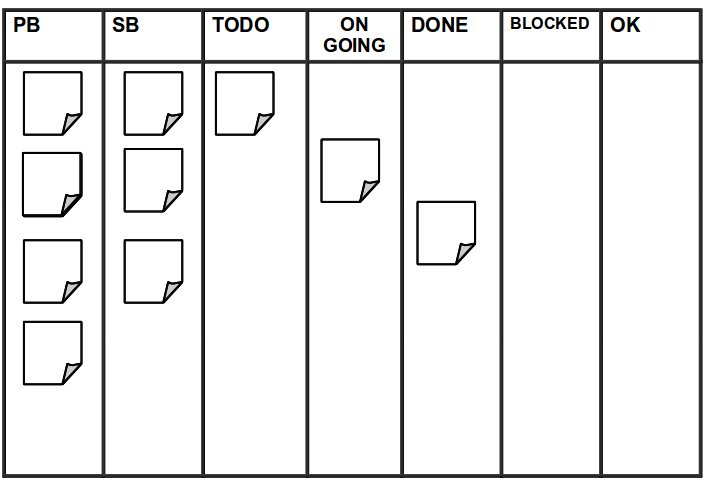
\includegraphics[width=0.9\textwidth]{ScrumKanbanBoard}
  \caption{Tablero Kanban para Scrum}
  \centering
  \label{fig:ScrumKanbanBoard} %\ref{fig:ScrumKanbanBoard}
\end{figure}

\subsubsection{Ejemplo de un Scrum board}

Un Scrum board, Kamban Board o taskboard físico (Ver figura \ref{fig:ScrumBoard}) es una tabla donde se colocan postick representando tareas.

\begin{figure}[h]
  \centering
  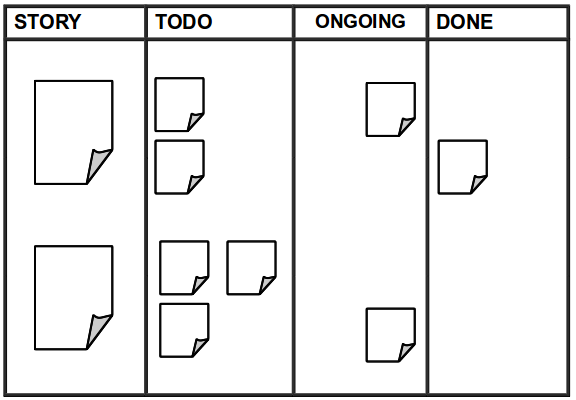
\includegraphics[width=0.8\textwidth]{ScrumBoard}
  \caption{Tablero Scrum}
  \centering
  \label{fig:ScrumBoard} %\ref{fig:ScrumBoard}
\end{figure}

